\documentclass[a4paper, 11pt]{book}
\usepackage[utf8]{inputenc}
\usepackage{minted}
\usepackage{graphicx}
\usepackage{hyperref}
\usepackage[linguistics]{forest}
\usepackage{bussproofs}

\newenvironment{bprooftree}
  {\leavevmode\hbox\bgroup}
  {\DisplayProof\egroup}
  
\hypersetup{
    colorlinks,
    linkcolor={red!50!black},
    citecolor={blue!50!black},
    urlcolor={blue!80!black}
}
\usepackage[backend=biber,style=alphabetic]{biblatex}
\DeclareUnicodeCharacter{2200}{$\forall$}
\addbibresource{hdr.bib}
\addbibresource{other.bib}

\DeclareSourcemap{
  \maps[datatype=bibtex, overwrite]{
    \map{
      \perdatasource{hdr.bib}
      \step[fieldset=keywords, fieldvalue={, }, appendstrict]
      \step[fieldset=keywords, fieldvalue=me, append]
    }
    \map{
      \perdatasource{other.bib}
      \step[fieldset=keywords, fieldvalue={, }, appendstrict]
      \step[fieldset=keywords, fieldvalue=they, append]
    }
  }
}
%'theorem.py:CoqLexer -x'
\newminted[elpicode]{'elpi.py:ElpiLexer -x'}{fontsize=\small,autogobble,escapeinside=~~,mathescape=true,frame=leftline,framerule=0pt,framesep=1em}
\newmintinline{elpi}{fontsize=\small,autogobble,escapeinside=~~,mathescape=true,frame=leftline,framerule=0pt,framesep=1em}
\newminted[coqcode]{'theorem.py:XCoqLexer -x'}{fontsize=\small,autogobble,escapeinside=~~,mathescape=true,frame=leftline,framerule=0pt,framesep=1em}
\newmintinline{coq}{fontsize=\small,autogobble,escapeinside=~~,mathescape=true,frame=leftline,framerule=0pt,framesep=1em}
 
\newenvironment{dedication}
  {%\clearpage           % we want a new page          %% I commented this
   \thispagestyle{empty}% no header and footer
   \vspace*{\stretch{1}}% some space at the top
   \itshape             % the text is in italics
   \raggedleft          % flush to the right margin
  }
  {\par % end the paragraph
   \vspace{\stretch{3}} % space at bottom is three times that at the top
   \clearpage           % finish off the page
  }
\title{Elpi: rule-based extension language}
\begin{document}
  
\chapter*{Dedication}
\begin{dedication}
To Cinzia and Anna
\end{dedication}

\setcounter{tocdepth}{5}
\tableofcontents

 \chapter{Introduction}


\section{Prologue}

\subsection{Beyond the odd order theorem}

I had the luck to be part of this project.
After its completion the good question was what it made it possible
other than having Georges Gonthier lead the project. How to make
it possible for others to build such an impressive machine checked
proof. I've always been interested into building tools, since I believe
a tool can democratize...

3 points 1) engineering practices, not new but too often
ignored by the community; 2) formalization technique known as boolean
reflection (or small scale reflection) that carves a light weight
``classical math'' framework in Coq (EM, UIP, FUNEXT) in Coq when
constructivism allows for it; 3) ``creative'' programming of the
Coq elaborator.

We focused on 3. These programs make Coq behave as an informed readers,
that is a reader that knows some base facts and that is expected to
be able to combine them using some well known rules. It was customary,
at that time, to see Coq as a ``dumb reader'': you have to explain
every single detail to him. These programs changed the game  for the
oothm and made it possible to use notations as in math, that is convoy
a lot of information implicitly, by convention.

The objective was to help users craft these programs. Programming
the elaborator as we did was hard. Structuring the library to that
knowledge could be organized by the author an retrieved by these
programs was even harder. The programming mechanism is called CS,
and is strictly related to the UH I studied during my PhD.
Independently, about at the same time,
Coq got extended with type classes, which happened to be usd for similar
purposes, and immediately raised similar programming issues.

To my eyes, these programs were strikingly related to Prolog.
Our programs were organized in rules and driven by unification.
At that time I had barely heard about Prolog.
It happened that the Parsifal team
at Inria Saclay worked on a language or that family
and thanks to Assia Mahboubi and Stephane Legrand I could give a talk
at a STTT workshop they were hosting.

In my talk I did explain some of the programs we wrote and why they
were helping us writing math in Coq. Dale Miller, asked a few questions
and suggested that his $\lambda$Prolog language was probably what I
was looking for, but since I did not know anything about it I could
just nod and ask to continue to the discussion offline.

not just the rules but also their animation and maybe also the entire
elab algorithm.

Dale was kind
to set up a meeting with Claudio Sacerdoti and myself. 

\subsection{The beginning: a snowy day}

On that day ``Paris'' was frozen, in the sense that a supposedly
``show storm'' convinced authorities to close buildings and other facilities,
reduce public transportations to the bare minimum. For some reasons
the XXX building was not closed, so the 3 of us agreed to buy a sandwich,
walk up the hill (with boots) and meet in a desert building.

After two hours of gentle introduction, after having savoured the
elegance of \elpiinline{copy}, I clearly remember I say ``sold...'',
but I also completed the sentence with ``how do I do evars?''.

$\lambda$Prolog could easily describe the rules my programs were
made of and elegantly manipulate the data type of Coq terms that
notably contains many binders. But also holes, evars in Coq slang,
that are the other beast one has to tame in order to implement an
elaborator and, in general, the outern layers of a toll like Coq.

It was the beginning.

Teyjus in bologna, we could write a toy elaborator in one day
but we could not find a good solution. Reification is ugly, one has
to pass a subst and reimplement unif. At the same time reusing unif
variables seemed possible, but extremely hard since the pure core
of LP, and Teyjus, do not really give you systems to control their
assignment and an elaborator takes in input a term with holes
and returns a term where only some holes are assigned...

It was worth trying but using teyjus in Matita or Coq was too hard.
I write a POC interpreter of LP in OCaml for embedding it into
Matita and Coq, elpi. It was easy to add hacks and experiment with
it, and that ... Elab in matita was kind of working, we could run
it on the arithmetic library. It was clear that:
the perf were bad, very bad, like 22K times bad.
the hacks could be explained in terms of constraints and rules to
suspend, resume, combined them.


\section{Elpi}
Elpi is both a language and an implementation of that language.

With CSC we rewrote the runtime, first the FO part then the HO part
and 

line stats

I perceived many times, in academic circles, some mistrust in logic programming.


We organize this document in four parts. The first two describe Elpi from
A to Z, both as a language and as an implementation of that language (we credit
\cite{ridoux1998lambda}). The third describes the integration of Elpi in Coq
and the fourth one surveys the application developed for Coq using Elpi.


\chapter{Elpi the language: \emph{de A \`a Z}}

Elpi is a mix of two languages: $\lambda$Prolog and Contraint Handling Rules.
The former is a higher order variant of Prolog based on
Hereditary Harrop Formulas, a generalization of Horn Clauses.
The latter is language to manipulate a store of constraints that,
in the case of Elpi, is made of suspended goals, i.e. sequents
made of heigenvariables, dynamic rules and a conjecture.

We briefly introduce all the ingredients that constitute Elpi.
Most of the syntax of Elpi is inherited from $\lambda$Prolog, as well
as the type discipline~\cite{Miller_Nadathur_2012}; similarly most of
its dynamic semantics is inherited from Prolog.
We state this upfront with no claim of novelty and but we just say Elpi in what
follows. We shall still highlight the novelties or simply differences from
$\lambda$Prolog or Prolog as they appear.

\section{Elpi v.s. Prolog}

Regarding an introduction to Prolog, the reader is spoiled for choice.
Here, we limit ourselves to establishing the terminology and highlighting
the key characteristics of Elpi and differences from standard Prolog from the
perspective of the programmer. We identify three of them: data types, rules
and search.

The first feature worth pointing out is algebraic data types, such as
list and trees. Here the declaration of binary tress in Elpi syntax:

\begin{elpicode}
kind tree type.
type leaf tree.
type node int -> tree -> tree -> tree. 
\end{elpicode}

The \elpiinline{leaf} and \elpiinline{node} function symbols can be used to
build ``compound terms'' and have arity 0 and 3 respectively. Elpi
follows the tradition of typed functional languages by prescribing not only
an arity but a more precise type to \elpiinline{leaf} and \elpiinline{node}.
In this document we refer to them as term constructors, or simply constructors.
Types play no role at run time but grately contribute to the static analysis
of the code, allowing to report typos and sometime even true errors early.

Here an example of the three

\begin{forest}
  [46 [93 [-] [-]] [-]]
\end{forest}

\begin{elpicode}
T = (tree 46 (tree 93 leaf leaf) leaf)
\end{elpicode}
  
To the reader familiar with
Prolog we point out that Elpi adopts the syntactic convention
of $\lambda$-calculus for function calls, namely $(f~ x~ y)$ rather than the
mathematical convention $f(x,y)$ adopted by Prolog.

The second feature we discuss is that the code is organized into
rules, that constitue the smallest code unit\footnote{In this document we prefer the
word rule to clause.}. A rule is made of two parts, the head and the premises.
Intuitively the head drives the selection of a rule, reducing the current
problem, that we goal, to simpler ones. Operationally the head is unified with the
goal, possibly assigning value to the rule parameters that are embodied by
unification variables. For example code computing the size of a tree, together
with its signature:

\begin{elpicode}
type size tree -> int -> prop.
size leaf 0.
size (node _ L R) N :- size L N1, size R N2, N is 1 + N1 + N2.
\end{elpicode}

Again we favor a type assignment to a simple arity. \elpiinline{prop} is the
type of executable code, meaning that \elpiinline{size}, when applied to two
arguments, becomes a goal and a program can be run to solve it.
On the contrary \elpiinline{node}, applied to any number of arguments,
is just a piece of data, it is not a goal.

\begin{elpicode}
goal> size T N.

Success
  N = 2
\end{elpicode}

Operations on built-in data types, such as integers, are provided via
the built-in \elpiinline{is} operator that evaluates its right hand side
and unifies the result with the left hand side.

It is worth pointing out that variables do not need to be used linearly
in the head of a rule: since the head is unified with the goal, it makes sense to
write there any therm, not just terms that happen to be patterns in
the sense of functional programming languages. For example the following
piece of code succeeds only if the tree is empty or made of two
identical subtrees.

\begin{elpicode}
type symmetric tree -> prop.
symmetric leaf.
symmetric (node _ T T).
\end{elpicode}

The third characteristic is that Elpi internalizes a form of search called
backtracking: all rules are potentially applied and there is no committment to
the first rule whose head unifies with the goal.
Here an example of code relying on backtracking to test
the membership of an element ot a tree.

\begin{elpicode}
type mem tree -> int -> prop.
mem (node N _ _) N.
mem (node _ L _) N :- mem L N.
mem (node _ _ R) N :- mem R N.
\end{elpicode}

Backtracking is a very powerful feature but without control leads to
unnecessarily bad computational complexity. The one contruct to control
backtracking is the cut operator.

\begin{elpicode}
mem (node N _ _) N :- !.
mem (node _ L _) N :- mem L N, !.
mem (node _ _ R) N :- mem R N.
\end{elpicode}  

Operationally the cut is not a premise to be solved, but rather telling
the runtime the intention to commit to the current rule and solution.
The former cut indicates that if the number is found in the current node
we commit to this rule and discard the following ones: we do not care
if the number also occurs deeped in the tree. The second cut indicates
that if the number was found in the left sub tree we shall not look in
the right sub tree so we discard the last rule\footnote{To be precise
the second cut also discard any alternative solution (yet to be computed)
to the preceeding premises. Technically speaking, Elpi implements a hard cut.}.

\subsection{What really matters (to us)}

Algebraic data types are an essential tool to write succint code
to describe and process syntax trees. They are available in languages
from the Prolog family, but also in most functional languages. Hence they do
not constitute the feature that tips the balance in favor of a logic
programming language.

On the contrary functional languages do not usually come with backtracking
while it is undeniable that logic programming and backtracking are linked by
a strong bond and that the ability to ``compute relations'' is a typical
selling point. Still, according to our experience, the vast majority of code
written in Elpi does not need this feature.

So, in conclusion, I believe that the most interesting
characteristic of logic programming is of being a rule based language.

It trades the elaborate syntax offered by most
programming languages with the notion of a smaller code unit.
A code unit has a meaning per se and the operation of adding or removing it
to/from a program is well defined.

An assignment, a while loop, or a function definition do not
constitute a code unit. An assignment is meaningless without a variable
declaration, similarly a while loop: they only get a meaning, even a formal 
one, in a larger context. Even the definition of a self contained function fails to be a unit in
this sense: while adding it to a program makes some sense (although, since nobody
calls it, serves little purpose),
removing a used function just results in a non functional program.

A rule has a meaning given by its logical interpretation. Adding it or removing
it from a logic program simply results in a different logic program. Typically
by adding a rule the resulting program is able to handle one more case,
a bit like a proof system lets you prove more statements if one poses
more axioms, or becomes more and more incomplete as axioms are removed.
From the parallel with proof systems it is obvious that adding ``bad'' rules
can result in a program that gives unexpected answers, but the operation
of adding or removing them is still meaningful, even if one admits non logical
constructs and departs for the ideal world of logic.
If we admit non logical
constructs then the order of rules becomes relevant and the insertion of a
rule better be accompanied by a grafting directive, like begin added before
or after another rule.

It it thanks to this rule-based nature that logic programming scales so
naturally to the domain of syntax trees with binders (next section)
and that it integrates so well with interactive provers (see~\ref{sec:rocq}).

\section{Elpi v.s. $\lambda$Prolog}

The syntax trees we are interested in are the ones that constitute
the foundational language of interactive provers like Coq. A characteristic common
to all of the them is the presence of binders, as forall and exists in
the world of specification or (lambda) abstraction in the world of terms.

The ``hello world'' example in this domain is simply typed lambda calculus,
a formalism now almost a century old. The syntax of terms and types
is declared as follows:

\begin{elpicode}
kind term type.
type lam (term -> term) -> term.
type app term -> term -> term.

kind ty.
type arr ty -> ty -> ty.
\end{elpicode}

The type declaration for terms introduces a pairing constructor \elpiinline{app},
putting together a function and its argument, and a function former
\elpiinline{lam} that abstracts a term over a (bound) variable representing the
formal argument. The declaration uses the function space of
the programming language in order to represent the abstraction:
the function carried by \elpiinline{lam} can be applied to an actual argument in order
to recoved the body of the expression where the formal argument is
replaced by the actual argument.

In this syntax the fst function is written as follows:

\begin{elpicode}
Fst = (lam x\ lam y\ x)
\end{elpicode}

Note that \elpiinline{(x\ lam y\ x)} is a function of \elpiinline{x} (a
variable of the Elpi programming language)
and that the syntax tree of our object language, $\lambda$-calculus, does not
feature a term constructor for variables since one can reuse the variables
of Elpi.
As sketched above the body of the first abstraction
can be recovered by applying the function: \elpiinline{((x\ lam y\ x) c)}
gives \elpiinline{(lam y\ c)}.


% \begin{elpicode}
% type copy term -> term -> prop.
% copy (lam F) (lam G) :- pi x\ copy x x => copy (F x) (G x).
% copy (app A B) (app C D) :- copy A C, copy B D.
% \end{elpicode}

The type checker for the simply typed $\lambda$-calculus can be implemented by
the following two rules:

\begin{elpicode}
type of term -> ty -> prop.
of (app H A) T :- of H (arr S T), of A S.
of (lam F) (arr S T) :- pi c\ of c S => of (F c) T.
\end{elpicode}

The rule for application reads: in order to assign type \elpiinline{T} to
the application of \elpiinline{H} to \elpiinline{A} we need to assign
the type \elpiinline{S} arrow \elpiinline{T} to \elpiinline{H} and
the type \elpiinline{S} to \elpiinline{A}. The one for abstraction
assigns the type \elpiinline{S} arrow \elpiinline{T} if, given any
fresh symbol \elpiinline{c} of type \elpiinline{S} the body of
the function \elpiinline{F} has type \elpiinline{T} when the bound variable
is substituted by \elpiinline{c}.


The two rules above closely match the ``inference rules'' commonly used in
by the logic or programming language communities:
$$
\begin{bprooftree}
  \AxiomC{$\Gamma \vdash H : S \to T$}
  \AxiomC{$\Gamma \vdash A : S$}
  \BinaryInfC{$\Gamma \vdash H~A : T$}
\end{bprooftree}
\qquad
\begin{bprooftree}
  \AxiomC{$\Gamma, c : S \vdash F[x/c] : T \quad c~\mathrm{fresh~in}~\Gamma$}
  \UnaryInfC{$\Gamma \vdash \lambda x.F : S \to T$}
\end{bprooftree}
$$

The main difference is that $\Gamma$ is managed by Elpi: the \elpiinline{pi}
operator guarantees the freshness of $c$, while \elpiinline{=>} augments
the current program with an instance of the rule:

$$
\begin{bprooftree}
  \AxiomC{$x : T \in \Gamma$}
  \UnaryInfC{$\Gamma \vdash x : T$}
\end{bprooftree}
$$

While Prolog finds it roots on Horn clauses, $\lambda$Prolog and hence
Elpi are based on Hereditary Harrop formulas~\cite{}. While the rule for application
can be seen as a formula in the Horn fragment:

$$
\mathrm{of}~ H~(\mathrm{arr}~S~T) \land \mathrm{of}~A~S \Rightarrow \mathrm{of}~(\mathrm{app}~H~A)~T
$$

\noindent the rule for lambd aabstraction truly needs the $\forall$ quantifier
and the use of (nested) implication:

$$
(\forall c, \mathrm{of}~c~S \Rightarrow  \mathrm{of}~(F~c)~T) \Rightarrow \mathrm{of}~(\mathrm{lam}~F)~(\mathrm{arr}~S~T)
$$

The reading of the rule for abstraction as an Hereditary Harrop formula
makes it clear that the scope of $c$ and the so called hypothetical rule
assigning it a type are limited to the subgoal $\mathrm{of}~(F~c)~T$,
unlike the \texttt{assert/1} and \texttt{retract/1} Prolog builtins\footnote{
  although some Prolog implementation provide the notion of ``transation''
that can be used to simulate scoping.}.

As previously announced, we want to use Elpi in the contet of an
interactive prover like Coq where syntax trees are often incomplete, i.e.
they contain holes. For example we would like to run the
type checker of this goal: \elpiinline{of (app F A) T}.

This is where $\lambda$Prolog falls short, by lack of a way to avoid
divergence by suspending search on certain goals and lack of a sub language
to manipulate suspended goals.


\subsection{Incomplete terms}

$\lambda$Prolog provides native support for syntax trees with bound
variables via the re-use of the function space of the programming language
to represent binders. This technique is called Higher Order Abstract Syntax,
or $\lambda$-tree syntax. The language also provides another kind
of variables, meta-variables actually, that we call unification variables.
These unification variables are equipped with a scope, a list of bound
variables that can be used in their assignment. This is essential to
avoid capturing variables by mistake, and it is well studiend in~\ref{}.

The natural question is: can we reuse the unification variables of
the programming language to represent holes in the syntax trees we manipulate?
In other words, the runtime of of our Logic programming language is already
carrying a substitution for these variables, undoing its application upon
backtracking, avoiding the generation of circular terms (i.e. not trees)
by performing occur check, and avoiding captures: can we reuse all that?

Elpi tries to give a positive answer to this question. Moreover it provides
support to attach data to holes ``on the side'', similarly to what
hypothetical rules are used for in the type checker above: attach a type
to fresh constants.

From a programming perspective, the needs are the following ones:

\begin{description}
  \item[control instantiation of holes] in particular be able to opt out of the
     generative behavior of Prolog based on the order of rules. According to
     our experience when a hole is encountered one of the following two
     actions need to be implemented: either suspend the computation and
     generate a constraint, or synthesize an assignment for the hole
     via a dedicated routine
  \item[attach data to holes] from a simple boolean flag, as we will do
    when implemeting ML type inference with equality types,
    to a full typing sequence as it is necessary to do when holes represent
    Coq terms

  \item[manipualte attached data] such as combine multiple data attached to the same
     hole or perform a consistency check when the hole gets assigned

\end{description}


\section{Modes and Constraints}

Elpi provides a notion of mode declaration that is uncommon to logic programming.
In particular arguments that are flagged as input are not required to be
ground in the goal, but are matched against the rule ``pattern'' instead 
of being unified. This means that no unification variable occurring in
the goal inside an input argument is instantiated when the rule is
fired.

Mode declaration comes together with the \elpiinline{uvar} keyword to denote
holes in the head of a rule.

In the light of that we can rephrase the type checker for simply typed $\lambda$-calculus
as follows:

\begin{elpicode}
pred of i:term, o:ty.
of (app H A) T :- of H (arr S T), of A S.
of (lam F) (arr S T) :- pi c\ of c S => of (F c) T.
of (uvar as E) T :- declare_constraint (of E T) [E].
\end{elpicode} 

The \elpiinline{pred} directive combines a type and mode declaration.
The \elpiinline{uvar as E} binds to the unification variable \elpiinline{E}
a hole in the goal and is semantically equivalent to the following,
where \elpiinline{var/1} is the standard Prolog predicate testing if
a variable is unbound.
  
\begin{elpicode}
of E T :- var E, declare_constraint (of E T) [E].
\end{elpicode}

Many Prolog implementations feature a ``delay directive'' sublanguage to
prescribe when goals should be suspended or resumed. In Elpi we opeted for
a more low level but also more flexible approach where the programmer declares
constraints / suspends goal via  the \elpiinline{declare_constraint} built-in
predicate. In the example above \elpiinline{[E]} is the list of variables
that ``block'' the suspended goal: as soon as one is assigned the goal should
be resumed.

It is worth pointing out that the input mode described above can in principle
we ``emulated'' via a program transformation that we sketch below:

\begin{elpicode}
of E T :- not (var E), E = (app H A), of H (arr S T), of A S.
of E (arr S T) :- not (var E), E = (lam F), pi c\ (of E S :- not (var E), E = c) => of (F c) T.
of E T :- var E, declare_constraint (of E T) [E].
\end{elpicode}

With this mechanism in place the type checker can do something useful
on terms containing holes:

\begin{elpicode}
goal> of (app H A) T.
Success:

Constraints:
  of A S  /* suspended on A */
  of H (arr S T)  /* suspended on H */
\end{elpicode}

The resumption 

\begin{elpicode}
goal> of (app H A) T, H = (lam x\ x).

Success:

Constraints:
  of A T  /* suspended on A */
\end{elpicode}

And the very same result is given on the goal \elpiinline{of (app (lam x\ x) A) T}.
  
Unfortunately the sole possibility of suspending and resuming goals is
not enough to implement a satisfactory type checker. An example of
goal giving an unexpected result is \elpiinline{of (app D D) T}
that succeeds with constraints

\begin{elpicode}
  of D S  /* suspended on D */
  of D (arr S T)  /* suspended on D */
\end{elpicode}

that are clearly incompatible.

We need a language to combine the constraints attached to hole \elpiinline{D}.

\section{Constraints Handling Rules}

A C.H.R.~\cite{chr}
program is a set of rules that maintain the constraint store, a
multi-set of (suspended) goals. A rule adds or removes constraints
from the store, and rules are applied following their order
as per the refined operational semantics~\cite{10.1007/978-3-540-27775-0_7}
of C.H.R.

The following Elpi code complements the running example by
imposing that each hole has only one typing constraint.

\begin{elpicode}
constraint of {
  rule (of X T1) \ (of X T2) <=> (T1 = T2)
}
\end{elpicode}

The rule reads: if the constraint \elpiinline{of X T1} is present
in the store together with \elpiinline{of X T2}, then remove
the latter and generate a new goal \elpiinline{T1 = T2}.
This is sufficient to make the type checker
reject \elpiinline{of (app D D) T}, since the goal
\elpiinline{S = arr S T} fails (because of occur check).

A detail to remak is that the constraints are matched against
the constraint handling rules, that is the non linear occurrence
of \elpiinline{X} does not risk to ``merge'' two unrelated constraints:
the rule above only applied if two constraint about the same variable
are in the stote.

Another important difference is that constraint handling rules
match more goals at once. While the execution of an Elpi program
can be seen as a depth-first construction of a proof tree, with
the possibility of suspending the exploration of a branch, the
application of a constraint handling rule operates on all suspended
branches. In a way it is a ``meta'' proof search step. It can for
example identify to identical subgoals and share/connect their (missing)
proof. Indeed CHR rules do have a logical reading.

\begin{elpicode}
    rule G1 \ G2 | T <=> G3
\end{elpicode}

This rule is sound if, somehow, if $T \land G1 \Rightarrow (G2 \Leftrightarrow G2)$
  
As we mentioned before Elpi automatically manages the context, that is
the set of fresh constants generated by \elpiinline{pi} and hypothetical
rules introduced by \elpiinline{=>}. As a result an Elpi goal is
not just a predicate $P$, but rather a sequent $E \triangleright  \Gamma \vdash P$
where $E$ is the set of fresh constants and $\Gamma$ the set of hypothetical rules.

The previous rule to model uniqueness of typing is hence incomplete
since the same hole can occur under different contexts. This more
elaborate version accepts different contexts and sets of fresh constants.

TODO explain S1 S2 \cite{joijgov}.

\begin{elpicode}
constraint of {
  rule (E1 :> G1 ?- of (uvar X S1) T1) \ (E2 :> G2 ?- of (uvar X S1) T2)
    <=> (T1 = T2)
}
\end{elpicode}

While correct for simple types this rule does not scale for a type
discipline like the one of Coq where terms can occur in types,
i.e. where the constants in S1 occur in T1, and S2 in T2. In this
richer setting comparing T1 and T2 in the disjoint union is incorrect,
one needs to relocate one term under the context of the other in order
to unify them (and avoid pruning, TODO example)

bla $E1 \uplus E2 \triangleright \emptyset \vdash G$ where $\uplus$.

The most precise constraint handling rule is the following one:

\begin{elpicode}
constraint of {
  rule (E1 :> G1 ?- of (uvar X S1) T1) \ (E2 :> G2 ?- of (uvar X S1) T2)
    | (relocate L1 L2 G1 G2 T2 T2')
    <=> (E1 :> G1 => T1 = T2)
}
\end{elpicode}

First, \elpiinline{uvar X S} is the syntax for the unification variable X
with scope S, where S is a list of constants. The guard of the rule $G$,
namely \elpiinline{relocate L1 L2 G1 G2 T2 T2'}, runs as a Elpi goal
$E1 \uplus E2 \triangleright \emptyset \vdash G$ where $\uplus$ denotes

TODO: Example of abs evars?

Constraints and CHR serve many purposes:
\begin{itemize}
  \item justify/implement some non-logical operations
  \item implement a state and its management
  \item schedule constraints
\end{itemize}

\section{Elpi = $\lambda$Prolog + CHR}

Elpi integrates the SLD search strategy typical of Prolog with
CHR as depicted:

%\begin{figure}
  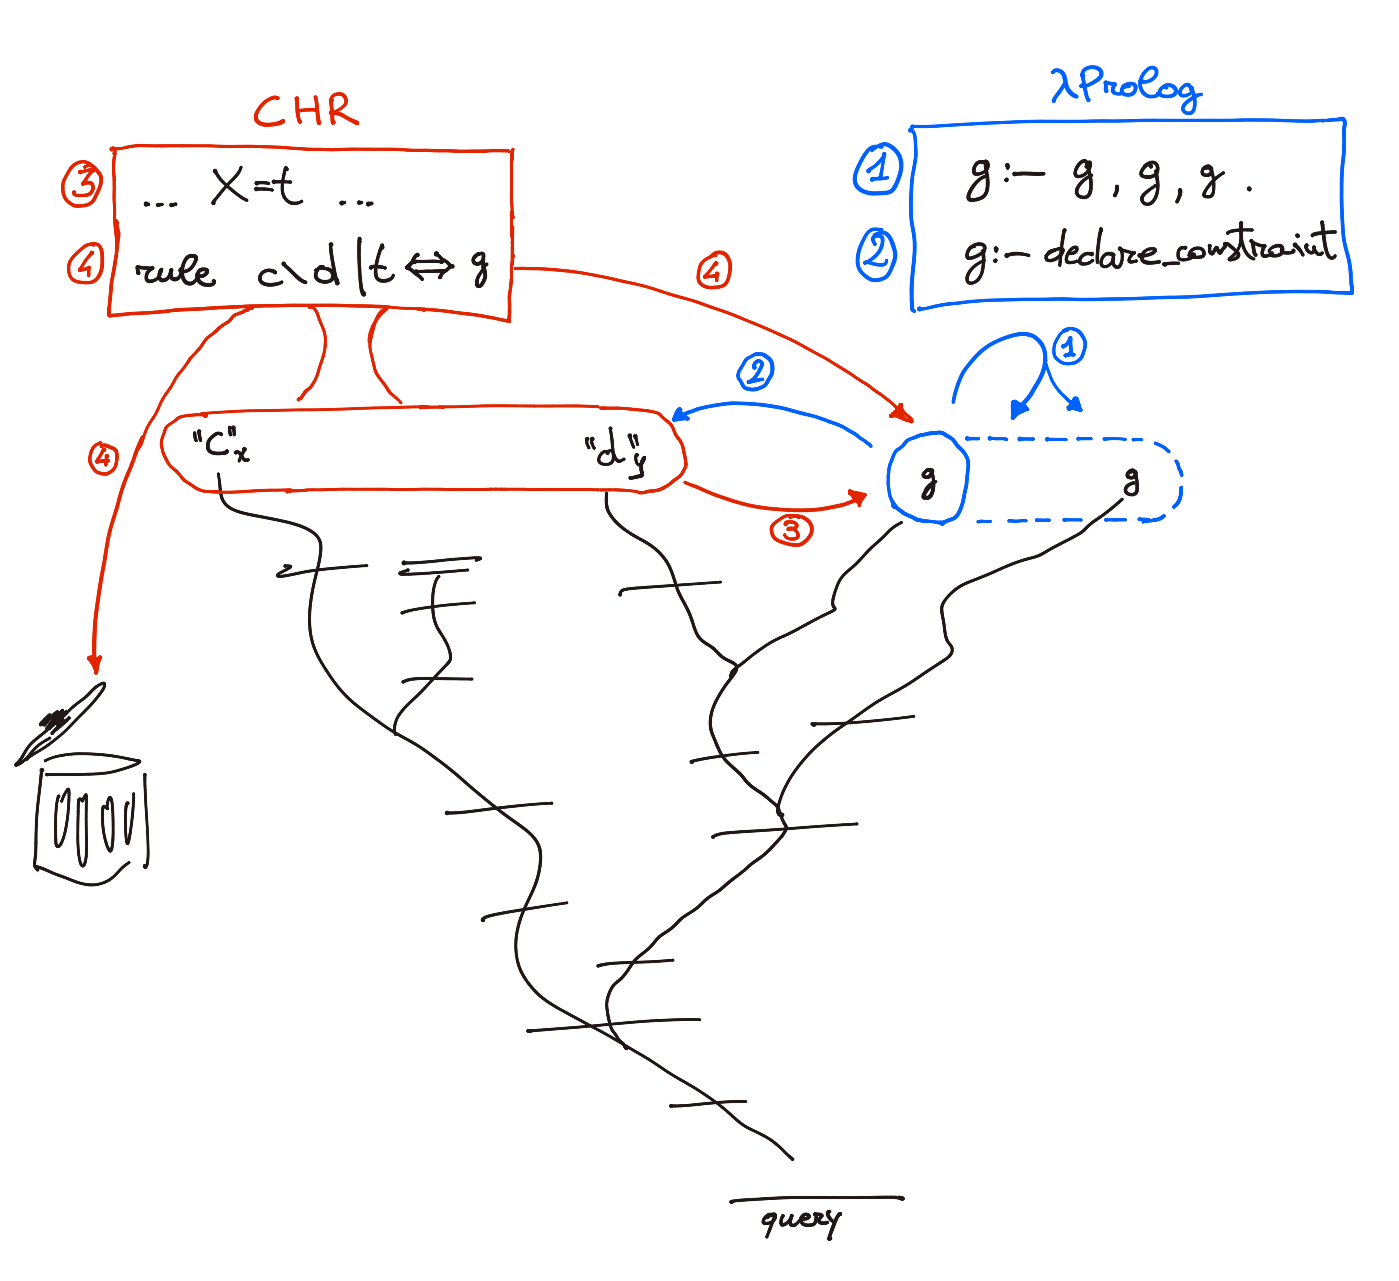
\includegraphics[width=0.8\textwidth]{chr.png}
%  \caption{\label{chr:fig}Elpi runtime (TODO clause/rule)}
%\end{figure}



 
Rule application follows the refined operational semantics~\cite{10.1007/978-3-540-27775-0_7}.
It amounts to precise neting of iterations. The starting point is
the so called ``active constraint'' $A$ that, in the context of Elpi, is
the constraint just declared via \elpiinline{declare_constraint}.

\begin{itemize}
\item for each rule $P_1 \ldots P_x \backslash P_{x+1} \ldots P_n | C \Leftarrow G$
\item for each position $0 < j \leq n$
\item for each permutation of $C_1 \ldots C_n$ constraints having $C_j = A$
\item match all $C_i$ with $P_i$ and run $C$. If it succeeds:
  \begin{itemize}
    \item remove $C_{x+1} \ldots C_n$ from $\mathcal{C}$
    \item remove all permutations involving $C_{x+1} \ldots C_n$
  \end{itemize}
\item move to the next rule
\end{itemize}

What may not be evident in the semantics above is the fact that the removal
of the active constraint 

\begin{elpicode}
  pred first.
  pred second.
  
  main :-
    print "declare first",
    declare_constraint first [_],
    print "declare second",
    declare_constraint second [_].
  
  constraint first second {
      rule second \ first <=> (print "rm first").
      rule first \ second <=> (print "rm second").
  }

  declare first
declare second
rm first

Success:

Time: 0.000

Constraints:
 second  /* suspended on X0 */
\end{elpicode}




\begin{elpicode}
pred first.
pred second.

main :-
  print "declare first",
  declare_constraint first [_],
  print "declare second",
  declare_constraint second [_].

constraint first second {
    rule second \ first <=> (print "rm first").
    rule        \ second <=> (print "rm second").
}
declare first
declare second
rm first
rm second
\end{elpicode}

\begin{elpicode}
pred c.

main :-
  print "declare first c",
  declare_constraint c [_],
  print "declare second c",
  declare_constraint c [_].

constraint c {
    rule c c <=> (print "rule 1").
    rule c <=> (print "rule 2").
}

declare first c
rule 2
declare second c
rule 1
rule 1
rule 2
\end{elpicode}



\section{Syntactic sugar}

Elpi features some simple syntactic sugar that is elimated by
the ``compiler'' before running programs.

\subsection{Namespaces}

Elpi code is obtained by accumulating together files, that is
``concatenating'' lists of rules, possibly written by different
authors. It is not impossible that
two files, file1 and file2, contain declarations for a predicate with same name p.

When the types for p do not match, Elpi fails immediately
and the programmer is warned. But when the types match, it may
happen that the predicate changes meaning or complexity,
especially in case of failure.

A simple man solution could be to simply put the file name
as part of predicate names, eg file1.p and file2.p.

To paliate the syntactic overhead Elpi provides two syntactic
facilities: namespace and shorten. The former prefixes all
names of the predicates contained in a block, the latter makes
predicates accessible via a short name inside a file or a block

\begin{elpicode}
namespace n1 {
  pred p.
}
\end{elpicode}

elsewhere

\begin{elpicode}
shorten n1.{ p }.
q :- p.
\end{elpicode}

note that a type/mode declaration declares the belonging to a namespace.

\begin{elpicode}
p.
namespace n2 {
  pred p.
  q :- p.
}
\end{elpicode}

\subsection{Spilling}

We argue that the names we give to the objects we manipulate
are the most important form of documentation and badly chosen
name are the primary cause of unreadable code.

The time a sloppy programmer saves by using \elpiinline{TMP}, \elpiinline{AUX}
or \elpiinline{X'} instead of thinking at an appropriate name is
demanded, with interests, to any reader of code, including himself.

Logic programming, even in its Higher Order flavor, distinguishes
commands from expressions (predicates from data). This characteristic
is the primary contributor to the proliferation of temporary
variables, a phenomenon that functional programming languages
reduce by putting in the same syntactic category function calls an
data. 

For example the OCaml code \texttt{List.rev (List.append l1 l2)}
or its equivalent \texttt{List.append l1 l2 |> List.rev} enables
to programmer to avoid naming the result of append, while in logic
programming one often reads

\begin{elpicode}
code L1 L2 Result :- append L1 L2 TMP, rev TMP Result.
\end{elpicode}

Elpi provides a syntatic facility to let one use
``partially applied'' predicates as ``function calls''.
By partially applied we mean ``applied to all the arguments flagged as input''.
For example the code above can be written as follows

\begin{elpicode}
code L1 L2 Result :- rev {append L1 L2} Result.
\end{elpicode}

The curly braces identify a term to be \emph{spilled} to the closest
\emph{execution point}, identified by walking the terms outside in and
identifying the first expression of type \elpiinline{prop}.

Spilling can be nested. Its elaboration is akin to the generation
of the administrative normal form that is commonly used in functional
programming languages.

\subsubsection{Spilling under a binder}

When the spilled expression needs to cross a binder in order to
reach the execution point, the elaboration is more sophisticated.
For example: 

\begin{elpicode}
code Result :- Result = (lam x\ {mk-app f [x]}).
code Result :- (pi y\ mk-app f [y] (TMP y)), Result = (lam x\ TMP x).
\end{elpicode}
  

In order to run the spilled code in a context with the bound variable
x, the expression must be put under a \elpiinline{pi y\\ }. Similarly
the temporary variable needs to be abstracted over the variable, so
that we can identify the original one x with the one abstracted by
\elpiinline{pi} y.

Note that spilling does not need to cross a \elpiinline{pi}, but
needs to make the quantified variable visible to the result of
the spilled computation, for example explicilty quantifying it
with a sigma. For example:

\begin{elpicode}
  code L1 L2 Result :- pi x\ rev {append [x|L1] L2} (Result x).
  code L1 L2 Result :- pi x\ sigma TMP\ append [x|L1] L2 TMP, rev TMP (Result x).
\end{elpicode}

\subsubsection{Spilling and impliction}

When the object language features a sophisticated HOAS for the context
(as in \ref{GALLINA}) it may be necessary to augment the context with
the implication operator. For example imagine the \elpiinline{lam}
term constructor carries the type of the bound variable

\begin{elpicode}
  code Ty Result :- Result = (lam Ty x\ lam {of x Ty => of (app g x)} y\ ...)
  code Ty Result :-
    (pi x\ of x Ty => of (app g x) (TMP x))
    Result = (lam Ty x\ lam (TMP x) y\ ...)
\end{elpicode}

This is frequent when spilling combined with quotations, for example

\begin{elpicode}
  T = {{ fun x : nat => lp:{{ app f {api x}  }}  }}
\end{elpicode}

where the api needs the context of the object language, see \ref{FFI}

\paragraph{Spilling ambiguities}

Not all that glitter is gold. Sometimes the closest execution
point may not be what the programmer wants.

\begin{elpicode}
  code D TodoForLater  :-
    TodoForLater [ this, that {rev D} ].
\end{elpicode}

If this and that are predicated, the latter becomes
\elpiinline{(rev D TMP, that TMP)} meaning that
D is reversed when TodoForLater will be executed, and
not when the todo list is generated, as one may have wanted.

According to our experience the closes execution point
is more often than not what the programmer expects.

\section{Example: Hindley Milner type inference}

the algorithm is meta since it needs to access the context and
in particular see the unassigned variables.

\begin{figure}
\begin{elpicode}
% terms
kind term type.
type global  string -> term.
type app term -> term -> term.
type lam (term -> term) -> term.
type let term -> ty -> (term -> term) -> term.
type eq  term -> term -> term.

% type expressions
kind tye type.
type (==>) tye -> tye -> tye.  

% types
kind ty type.
type all    eq? -> (tye -> ty) -> ty.
type mono   tye -> ty.

% type quantification
kind eq? type.
type any eq?. % any type
type eqt eq?. % type with an equality test

% builtin types
type int   tye.
type bool  tye.
type list  tye -> tye.
type pair  tye -> tye -> tye.
\end{elpicode}
\caption[syntax]{Syntax of terms and types\label{hm:syntax}}
\end{figure}


\begin{figure}
\begin{elpicode}
pred of i:term, o:ty.
of (global "1")      (mono int).
of (global "2")      (mono int).
of (global "3")      (mono int).
of (global "plus")   (mono (int ==> int ==> int)).
of (global "[]")    (all any x\ mono (list x)).
of (global "::")    (all any x\ mono (x ==> list x ==> list x)).
of (global "size")  (all any x\ mono (list x ==> int)).
of (global "undup") (all eqt x\ mono (list x ==> list x)).
of (global ",")     (all any x\ all any y\ mono (x ==> y ==> (pair x y))).
\end{elpicode}
\caption[type assignments]{Type assignments\label{hm:env}}
\end{figure}
  
\begin{figure}
\begin{elpicode}
pred specialize i:ty, o:tye.
specialize (mono T) T.
specialize (all any F) T :- specialize (F Fresh_) T.
specialize (all eqt F) T :- specialize (F Fresh) T, eqbar Fresh.

pred eqbar i:tye.
eqbar bool.
eqbar int.
eqbar (list A) :- eqbar A.
eqbar (pair A B) :- eqbar A, eqbar B.

eqbar T :- var T, new_constraint (eqbar T) [T,_].
eqbar T :- print "KO: type" T "has no equality", halt.
\end{elpicode}
\caption[schema elimination]{Type schema elimination\label{hm:elim}}
\end{figure}

\begin{figure}
\begin{elpicode}
% theta carries the list of type variables for which eqbar
% has to hold
pred theta i:list tye.
theta L :- new_constraint (theta L) [_].

% gammabar is not a real constraint, but rather a query to the meta
% level to compute a polymorphic type out of a monomorphic one and
% its context
pred gammabar i:ty, o:ty.
gammabar (mono T) TS :- new_constraint (gammabar (mono T) TS) [_].

% constraint store %
constraint of gammabar eqbar theta {
  rule (theta L)                    % matched
        \  (G ?- gammabar T TS)     % matched and removed
        |  (generalize L G T POLYT) % guard + syntesis
      <=> (TS = POLYT).             % new goal

  rule (eqbar V) \ (theta L) | (not(mem L V)) <=> (theta [V | L]).
}

pred generalize i:list tye, i:list prop, i:ty, o:ty.
generalize Theta Gamma (mono T) PolyT :-
  free-ty (mono T) [] VT,
  free-gamma Gamma [] VGamma,
  filter VT (x\ not(mem VGamma x)) ToQuantify,
  bind ToQuantify Theta T PolyT.

pred bind i:list tye, i:list tye, i:tye, o:ty.
bind [] _ T (mono T1) :- copy T T1.
bind [X|XS] Theta T (all E x\ T1 x) :-
  if (mem Theta X) (E = eqt) (E = any),
  pi c\ copy X c => bind XS Theta T (T1 c).

pred free-ty i:ty, i:list tye, o:list tye.
free-ty (mono X) L L1 :- free X L L1.
free-ty (all _ F) L L1 :- pi x\ free-ty (F x) L L1.

pred free-gamma i:list prop, i:list tye, o:list tye.
free-gamma [] L L.
free-gamma [of _ T|X] L L2 :- free-ty T L L1, free-gamma X L1 L2.

pred free i:tye, i:list tye, o:list tye.
free int L L.
free bool L L.
free (list A) L L1 :- free A L L1.
free (pair A B) L L2 :- free A L L1, free B L1 L2.
free (A ==> B) L L2 :- free A L L1, free B L1 L2.
free (uvar _ _ as X) L L1 :- if (mem L X) (L1 = L) (L1 = [X|L]).
\end{elpicode}
\caption[schema introduction]{Type schema introduction\label{hm:intro}}
\end{figure}


\begin{figure}
\begin{elpicode}
of (app H A) (mono T) :-
  of H (mono (S ==> T)),
  of A (mono S).

of (lam F) (mono (S ==> T)) :-
  pi x\ of x (mono S) => of (F x) (mono T).

of (let E PT B) (mono TB) :-
  of E (mono T),
  gammabar (mono T) PT,
  pi x\ of x PT => of (B x) (mono TB).

of (eq LHS RHS) (mono bool) :-
  of LHS (mono T),
  of RHS (mono T),
  eqbar T.

of X (mono T) :- of X (all E Poly), specialize (all E Poly) T.
\end{elpicode}
\caption[bidirectional]{Bidirectional typing\label{hm:bidir}}
\end{figure}

\begin{figure}
\begin{elpicode}
of (app H A) (mono T) :-
  of H (mono TH),
  of A (mono TA),
  assert H TH (TA ==> T).

of (lam F) (mono (S ==> T)) :-
  pi x\ of x (mono S1) => of (F x) (mono T1),
  assert (lam F) (S1 ==> T1) (S ==> T).

of (let E PT B) (mono TB) :-
  of E (mono T),
  gammabar (mono T) PT,
  pi x\ of x PT => of (B x) (mono TB1),
  assert (B x) TB1 TB.

of (eq LHS RHS) (mono B) :-
  of LHS (mono TL),
  of RHS (mono TR),
  eqbar TL,
  assert RHS TR TL,
  assert (eq LHS RHS) bool B.

of X (mono T) :- of X (all E Poly), specialize (all E Poly) T1, assert X T1 T.

pred assert i:term, i:tye, i:tye.
assert _ TY ETY :- TY = ETY, !.
assert T TY ETY :-
  print "KO: term" T "has type" TY "but its context expects" ETY, halt.
\end{elpicode}
\caption[monodirectional]{Monodirectional typing\label{hm:mono}}
\end{figure}


\section{Pitfalls}

During these years we gave Elpi in the hands of a
good number of users. Here the pitfalls that tricked everybody.

\subsection{precedence of \elpiinline{=>}}

When one write \elpiinline{A, B => C, D} means
\elpiinline{A, B => (C, D)}. This is clear when
one has a program \elpiinline{A, B => D} and wants
to sneak in a print to debug before D.

So we argue that => should bind stronger than ,
on the left but not on the right, something parsing
technology does not support out of the box. We introduced
==> that parses with these precedences and add a warning
whenever \elpiinline{A, B => C, D} that can be silenced
by writing \elpiinline{A, (B => C), D}.

\subsection{anonymous clauses}

HO lets one write \elpiinline{map L (x\r\p x A, q A r) L'}
where A is quantified (allocated) in the wrong place.
The correct way is \elpiinline{map L (x\r\sigma A\p x A, q A r) L'},
but we believe it would be way safer to only allow (partially
applied) predicates as HO arguments.

The syntactic overhead is often compensated by the extra
reading clarity a (well) named predicate provides.

\subsection{restriction failure as failure}

While \elpiinline{pi x\ F = x} clearly fails because x is
out of scope, its practical, legit, use cases are rare.
Most of the times when a unification fails because of
a scope problem, it is dues to a user mistake.

Although we have not tries to implement any measure to help
newcomers, we wonder if making this cause of unification failure
fatal (as is aborting the program) would help newcomers.


\chapter{Elpi the software: \emph{de A \`a Z}}

\section{The first prototype}

The first elpi was written by Tassi in about 3 months, with the objective
of understanding the $\lambda$Prolog language and some of the techniques
adopted to implement it, like the suspension calculus. This was elpi-POC

Terms were purely functional, to ease backtracking. This feature comes
with a reputation of making things hard, so we played conservative.

Suspension calculus did look similar to exp-substitutions, but until the very
last last paper in the pile on my desk it was not clear is was actually isomorphic
to $\lambda_\rho$. While explicit substitutions are often presented as a way to
obtain better performances, in practice they fail to deliver. In Coq two
people tried. In elpi-POC, in our limited tests, disabling them resulted in
a faster runtime.  bla bla about lazyness.

Elpi-POC was an easy playground to understand which features were needed in
order to manipulate terms with holes: a safeguard against instantiating them by
mistake (modes) and a was to attach metadata to holes (constraints).

Elpi-POC was functional enough to let us write an elaborator for CIC
and plug it into Matita. It was working, but it was too slow. Line 20K times
slower than reasonable.

Reason number one was the purely functional heap, with no GC. Introducing 
instructions to clear memory (in an unsafe way) was enough to see order of
magnitude fade.

\section{Second attempt: a runtime for $L_{\lambda}^{\beta}$}

imperative terms with a trail did not cause bugs, but a sensible speedup.
DBL made HO code sensibly faster \cite{dunchev15lpar}.

\subsection{The $L_{\lambda}$ fragment}
\subsection{The $L_{\lambda}^{\beta}$ fragment}

\cite{Michaylov1993HigherOrderLP}

built in lists.

CHR is still naive.

The compiler performs very little optimizations. In recent years its speed
in extending existing programs became relevant, since state is encoded as rules.

\subsection{Indexing}
\subsubsection{Patricial tree (over bits)}

predicate to index
symbol to clauses

special bucket for flex arg or flex input arg

\subsubsection{Hash map}

multiple arg, variable depth. similar perf


\section{The API}

The APIs to drive the interpreter essentially lets one parse code, comile into
unit, assemble units and run it.

In addition to that and FFI and quotations

\subsection{Quotations}

the one rule is that a variable is bound in one language and only
one.

example from the tutorial

\subsection{FFI}\label{FFI}

FFI is akin to printf, given a first class description of
the types of the arguments it performs the conversion
back and forth.

The peculiarity is that the context and constraint store
is given too to the conversion functions. In particular
this enables a tight integration see \ref{GALLINA}.

the FFI makes extensive use of GADTs.

contextual conversion

\section{Debugging}

The first debug tool is print, and spy.

\begin{elpicode}
pred std.spy i:pred.
std.spy P :- print "enter" P, P, "exit" P.
std.spy P :- print "fail" P.
\end{elpicode}

This is simple, but very often sufficient.
The main downside of requiring altering the code, hence has impedence
of debugging distant code.

The runtime of elpi has a debuggin facility based on conditional compilation,
the runtime is compiled twice, once with instrumentation.
The instrumentation was important to debug the runtime itself
but while it became more correct we added entry points for the user.

A post processing tool analyzes the trace reconstructung the
stack and generating data suitable to display an interactive navigation

\subsection{Trace browser}

screenshot

developed by Julien Wintz, it displays a trace as a mailbox of events
each events has pointers forward, backward and at a distance.
Each goal displays it full success or failure letting one
peek. The trace is searchable.

\chapter{Coq-Elpi}

While Elpi is a standalone language and software project, it was designed to
play the role of an \emph{extension language} for Coq. The glue between Elpi and
Coq is called Coq-Elpi.

My definition of this role, \emph{extension language}, is largely influenced
by the Lua programming language~\cite{10.5555/1200583}. Lua is an extension
language for applications written in C and is widely used in the Opens Source
world and in the gaming industry.
Its purpose is to provide an easy way to extend the host application.
It is easy to host Lua since its FFI is well curated, and thanks to that
exposing the internals of the application to the extension language requires a
limited effort to the application developer. It is easier to program in Lua,
rather than C, because the language is higher level, e.g. is features automatic
memory management and provides dictionaries as a builtin data structure.
Finally, it is easy for a user to get started with Lua because he does not need
to set up a proper development environment, the host application is sufficient
since Lua is an interpreter.\\
Elpi tries to do the same for OCaml, and Coq is the host application of interest.

Even if I'm not a big fan of it, in academia the same role is often called
meta-programming framework. Coq's main data type, terms, are programs and Elpi
programs do manipulate Coq programs. In this sense Elpi programs live at the
meta level.

\section{Why extending Coq in OCaml is hard}

Luckily OCaml features automatic memory management, types and algebraic data.
It is much, much higher level than C. Why it is hard to extend Coq then?

The first difficulty is that the complexity of the main Coq data type, terms,
is not completely hidden by the algebraic data types provided by the programming
language. The missing features are encoded and it is hard to completely hide
it to the programer (via curated APIs). In particular Coq terms feature binders
and holes. 

Binders pose two problems of their own and interact badly with holes.
The first problem is that they are typically encoded with numbers, De Bruijn
indexes, and it is just too easy to forget to shift a term.  The second program
is that when a binder is crossed on must always remember something about it,
typically the type of the bound variable. Hence the programs have to pass around
typing contexts (aka environment). It is tempting to not do it upfront, but
then one has to be disciplined. find mantra mc bride.

Holes are missing subterms and they come with metadata, a sequent.
Since the same hole can occur non linearly a single sequent is stored on the side of terms.
Moreover since binders may be reduced away each occurrence has an explicit
substitution. So there is a state that accompanies the terms, a state to be
threaded in a functional setting. This state also gathers univ constraints.
Assignment also part of this state, see also ``evar sensitive''. This is
a reified heap, we are back at memory management, pointer dereferencing (with no
types), no gc. The only thing that is easy is backracking, since the map is
purely functional.

The second difficulty is no inherent in OCaml, but rather an artifact of the
history of Coq. The API are not curated. Exposing the API in a manual, althought
not very demanding, way is key to rationalize them.


Last setting up the dev environment. I believe that can be eased with doc, but
there is another advantage in a interpreter, that you can iterate faster. Eg
in OCaml loading code is possible, but not unloading. This is even better in
a rule based language where far from the place where a code is written one
can add a rule to mask/improve/debug a piece of code.

\section{HOAS of terms and contexts}\label{GALLINA}

\begin{figure}
\begin{elpicode}
% Global objects: inductive types, inductive constructors, definitions
kind gref type.
type const constant -> gref. % Nat.add, List.append, ...
type indt inductive -> gref. % nat, list, ...
type indc constructor -> gref. % O, S, nil, cons, ...

kind term type.

type sort  sort -> term. % Prop, Type@{i}

% constants: inductive types, inductive constructors, definitions
type global gref -> term.
type pglobal gref -> univ-instance -> term.

% binders: to form functions, arities and local definitions
type fun  name -> term -> (term -> term) -> term.         % fun x : t =>
type prod name -> term -> (term -> term) -> term.         % forall x : t,
type let  name -> term -> term -> (term -> term) -> term. % let x : T := v in

% other term formers: function application, pattern matching and recursion
type app   list term -> term.                   % app [hd|args]
type match term -> term -> list term -> term.   % match t p [branch])
type fix   name -> int -> term -> (term -> term) -> term. % fix name rno ty bo

type primitive primitive-value -> term.
\end{elpicode}
\caption[terms]{Terms\label{hoas:term}}
\end{figure}
  
\begin{figure}
\begin{elpicode}
pred decl i:term, o:name, o:term. % Var Name Ty
pred def  i:term, o:name, o:term, o:term. % Var Name Ty Bo
\end{elpicode}
\caption[context]{Context\label{hoas:context}}
\end{figure}

\section{HOAS of holes (missing terms)}

holes come with data expressing an invariant
invariant checked when the hole materializes


\begin{figure}
\begin{elpicode}
pred evar i:term, i:term, o:term. % Evar Ty RefinedSolution
evar X Ty R :- not(var R), !, coq.typecheck R Ty ok, X = R.
 
constraint declare-evar evar def decl {

% Override the actual context
rule \ (declare-evar Ctx RawEv Ty Ev) <=> (Ctx => evar RawEv Ty Ev).
   
}
\end{elpicode}
\caption[holes]{Holes\label{hoas:holes}}
\end{figure}

%%%%%%%%%%%%%%%%%%%%%%%%%%%%%%%%%%%%%%%%%%%%%%%%%%%%%%%%%%%%%%%%%%%%%%%%%%%%%%%
%%%%%%%%%%%%%%%%%%%%%%%%%%%%%%%%%%%%%%%%%%%%%%%%%%%%%%%%%%%%%%%%%%%%%%%%%%%%%%%
%%%%%%%%%%%%%%%%%%%%%%%%%%%%%%%%%%%%%%%%%%%%%%%%%%%%%%%%%%%%%%%%%%%%%%%%%%%%%%


\section{Vernacular language integration}

While the language of Coq terms, gallina, is central to Coq-Elpi, there is another
language we have to describe first, the vernacular. That ``outern'' language
lets one organize the formalized knowledge, in particular give names to terms
and attach to them meta data.

Coq-Elpi extends the vernacular language with a few commands to declare, run
and modify Elpi programs.



\begin{figure}
\begin{coqcode}
Elpi Command hello.
Elpi Accumulate lp:{{
  main [str X] :- coq.say "Hello" X.
}}.
Elpi hello "reader".

Fail Elpi hello 46.

Elpi Accumulate lp:{{
  main [int X] :- coq.say "Hello" X.
}}.

Elpi hello 46.
\end{coqcode}
\caption[Vernacular]{Vernacular\label{vernac}}
\end{figure}

\subsection{Database, homoiconicity and rules}

share data between programs, and programmatically add data.

maybe later?

one feature that may not look evident is that
this is allowed (unlike in teyjus)
\begin{elpicode}
build C, C => more
\end{elpicode}

and that one can actually write build

\begin{elpicode}
build F H 0 (p F :- H).
build F H N (pi x \ C x) :-
  pi x\ 
    M is N - 1,
    build (app F x) M (p x,H) (C x).
\end{elpicode}


\section{Example: to bool}

\begin{figure}
  \begin{coqcode}
    From Coq Require Import Bool ssreflect ssrbool.
From elpi Require Import elpi.
Set Printing Coercions.

Axiom is_even : nat -> Prop.

Fixpoint even n : bool :=
  match n with
  | O => true
  | S (S n) => even n
  | _ => false
  end.

Lemma evenP n : reflect (is_even n) (even n).
Admitted.

Lemma andP  {P Q : Prop} {p q : bool} :
  reflect P p -> reflect Q q ->
    reflect (P /\ Q) (p && q).
Admitted.

Lemma elimT {P b} :
  reflect P b -> b = true ->
    P.
Admitted.

Elpi Db tb.db lp:{{
% [tb P R] finds R : reflect P p
pred tb i:term, o:term.

:name "tb:fail"
tb Ty _ :- coq.error "Cannot solve" {coq.term->string Ty}.

}}.

Elpi Tactic to_bool.
Elpi Accumulate Db tb.db.
Elpi Accumulate lp:{{

solve (goal Ctx _ Ty _ _ as G) GL :-
  tb Ty P,
  refine {{ elimT lp:P _ }} G GL.

}}.

Elpi Command add_tb.
Elpi Accumulate Db tb.db.
Elpi Accumulate lp:{{

% evenP : forall n, reflect (is_even n) (even N).
%
% tb {{ is_even lp:N }} {{ evenP lp:N }}.
%
% pi N\ tb {{ is_even lp:N }} {{ evenP lp:N }} :- [].

% andP : forall P Q p p, reflect P p -> reflect Q q ->
%                           reflect (P /\ Q) (p && q).
%
% tb {{ lp:P /\ lp:Q }} {{ andP lp:PP lp:QQ }} :-
%   tb P PP, tb Q QQ.
%
% pi P Q PP QQ\
%   tb {{ lp:P /\ lp:Q }} {{ andP lp:PP lp:QQ }} :-
%     [tb P PP, tb Q QQ].

pred compile i:term, i:term, i:list prop, o:prop.
compile {{ reflect lp:Ty _ }} P Hyps (tb Ty P :- Hyps).
compile {{ reflect lp:S _ -> lp:T }} P Hyps (pi h\ C h) :-
  pi h\
    compile T {{ lp:P lp:h }} [tb S h|Hyps] (C h).
compile {{ forall x, lp:(T x) }} P Hyps (pi h\ C h) :-
  pi x\
    compile (T x) {{ lp:P lp:x }} Hyps (C x).
    
main [str S] :-
  coq.locate S GR,
  coq.env.typeof GR Ty,
  compile Ty (global GR) [] C,
  coq.elpi.accumulate _ "tb.db" (clause _ (before "tb:fail") C).

}}.

Elpi add_tb evenP.
Elpi add_tb andP.

Elpi Print to_bool "Demo.snippets/to_bool".


Lemma test : is_even 6 /\ is_even 4.
elpi to_bool.
simpl.
trivial.
Qed.

  \end{coqcode}
  \caption[Databases]{Databases\label{databases}}
  \end{figure}

  
\chapter{Coq applications}

In this chapter we survey the main applications developed on top of Coq-Elpi.

\section{Derive}

The ``derive'' application is a framework to register automatic
code generation, typically in response to the declaration of a new inductive
data type.

Coq itself is known to generate induction principles and equality tests.
Unfortunately it is also known to generate bad induction principles when
containers (e.g. lists) are involved and often fail to generate useful
equality tests.

I saw the opportunity to improve on that starting with the L3 internship of
Luc Chabassier that wrote the first prototype in the summer of 2017.
He succeeded in generating
equality tests and their proofs in two months. While most of the credit goes to
his learning skills, the experience confirmed that Coq-Elpi was to support
research in this domain. Indeed the solution implemented by Luc, although
correct, was not very satisfactory since it was not very modular. Improving
on that lead to \cite{tassi:hal-01897468}, but before that I need to introduce
the swiss army knife of boilerplate code generation: parametricity.

\subsection{Parametricity}

The so called parametricy translation \cite{keller_et_al:LIPIcs.CSL.2012.381}
is a family of procedures that given \emph{any} Coq term $t$ of type $r$
give both a predicate $R$ and a proof $T$ that $R$ holds for $t$, that is $T : R~t$
in the unary case. For example the unary parametricity translation of
\coqinline{nat : U} is \coqinline{is_nat : nat → U} and
the translation of \coqinline{3} if a proof that \coqinline{is_nat 3} (we write
\coqinline{U} for the universe, e.g. \coqinline{Prop}).

The translation becomes interesting when the type has parameters such as
\coqinline{A} in \coqinline{list A}. In that case the translation builds
terms and type parametric in \coqinline{A} and in its translation. For example
the translation of \coqinline{list A} is a predicate
\coqinline{is_list : ∀A, (A → U) → (list A → U)},
and the translation of \coqinline{cons : ∀A, A → list A → list A} is
\begin{coqcode}
is_cons : ∀A (isA : A → U),
  ∀(a : A), isA a →
  ∀l, is_list A isA l →
    is_list A isA l
\end{coqcode}

The unary parametric of a container type is a predicate that
asserts that each term contained has a given property, \coqinline{isA}
in the example above. The unary parametricity translation is key to express in a
systematic way that a property holds deep inside a container.

The parametricity translation is meta, it cannot be implemented in Gallina
itself hence one needs a meta language to implement it. Its implementation
in Coq-Elpi was done by Cohen Cyril in the fall of 2017, as he was interested
in exploiting the binary version of the translation to transfer properties
automatically, possibly in the context of the Coq-EAL project.


\subsection{Deep induction}

Deep induction principles are said ``deep'' in contrast to the ones generated
by Coq that, in the presence of containers, are shallow (and proof theoretically
weak). As an example we can take the data type of rose trees.

\begin{coqcode}
Inductive rtree A : U :=
| Leaf (a : A)
| Node (l : list (rtree A)).
\end{coqcode}

The induction principle generated by Coq is

\begin{coqcode}
Lemma rtree_ind : ∀A (P : rtree A → U),
  (∀a : A, P (Leaf A a)) →
  (∀l : list (rtree A), P (Node A l)) →
  ∀t : rtree A, P t.
\end{coqcode}

That is weak since no element of \coqinline{l} in \coqinline{Node A l}
verifies \coqinline{P}. In \cite{tassi:hal-01897468} I study the synthesis
for a stronger principle where \coqinline{P} holds ``deep'' inside \coqinline{l}.

\begin{coqcode}
Lemma rtree_induction A is_A (P : rtree A → U) :
  (∀a, is_A a → P (Leaf A a)) →
  (∀l, is_list (rtree A) P l → P (Node A l)) →
     ∀t, is_rtree A is_A t → P t.
\end{coqcode}

There are two characteristics of this principle worth analyzing.

First and foremost it is deep since the assumption
\coqinline{is_list (rtree A) P l} gives access to \coqinline{P} on all
elements of \coqinline{l}.
In order to access \coqinline{P} one can combine lemmas such as
\begin{coqcode}
Lemma is_list_funct A P Q : (∀ a, P a → Q a) → ∀ l, is_list A P l → is_list A Q l.
\end{coqcode}

with the induction principle of the container
\begin{coqcode}
Lemma list_induction A (is_A: A → U) (P: list A → U):
  P nil →
  (∀ a (pa : is_A a) l, P l → P (a :: l)) →
  ∀ l, is_list A is_A l → P l.
\end{coqcode}

Note how the former works under \coqinline{is_list} while the latter eliminates it.

\begin{coqcode}
Definition rtree_induction (A : U) (PA : A → U) (P : rtree A → U)
  (His_Leaf : ∀a : A, PA a → P (Leaf A a))
  (His_Node : ∀l : list (rtree A), is_list (rtree A) P l → P (Node A l)) :=
  fix IH (s1 : rtree A) (x : is_rtree A PA s1) {struct x} : P s1 :=
  match x in (is_rtree _ _ s2) return (P s2) with
  | is_Leaf _ _ a Pa => His_Leaf a Pa
  | is_Node _ _ l Pl => His_Node l (is_list_functor (rtree A) (is_rtree A PA) P IH l Pl)
  end.
\end{coqcode}


In a way the induction principle states that ``if a term is of type t then it validates P''


\subsection{Natural equality tests}

Once one has induction principles he can prove properties about recursive programs.
The first is equality test.

\begin{coqcode}
Definition rtree_eq A (A_eq : A → A → bool) :=
  fix rec (t1 t2 : rtree A) {struct t1} : bool :=
  match t1, t2 with
  | Leaf a, Leaf b => A_eq a b
  | Node l, Node s => list_eq (rtree A) rec l s
  | _, _ => false
  end.
\end{coqcode}



\cite{tassi:hal-01897468}

\subsection{Fast equality tests}

This is OK but terms are quadratic

\cite{gregoire:hal-03800154}


\section{Hierarchy Builder}

The math comp library has many good points and a few bad ones. Among these
the most endangering ons is that the barrier to entry is high. Documentation
a in \cite{assia_mahboubi_2022_7118596} helps, but any motivated learner
can only read so much. In particular the last chapters of the book above
quickly grow in complexity and technicality. The problem is that, prior to
HB, defining a hierarchy of algebraics structure à la mathcomp was terribly
hard. So hard that I myself would have not get it right at the first try.

In Spring 2019 Cohen Cyril came back from a Dagstuhl seminar with ``a language for
describing the math-comp hierarchy''. He needed a way to implement his language and
Coq-Elpi had almost all the features he needed: APIs to declare records and
canonical structure instances.

To be honest, at that time Coq-Elpi lacked so many features, but the objective
at stake was both a strong motivation for adding them and also a good test
bench for their implementation.



\cite{cohen_et_al:LIPIcs.FSCD.2020.34}

\subsection{Mathematical Components 2.0}

Porting Mc to HB was a huge effort. we did it with a sprint.

\cite{affeldt:hal-03463762}

\includegraphics[width=\textwidth]{hb\_intf.png}

one should remark that not only MC2 has the same interfaces, but
also that the trend changed, much more are defined.

MCa has 64 + 24 legacy, as of 1.2.0-8-g1baa0a8


% mathcomp-1.6.1 mathcomp-1.7.0 mathcomp-1.8.0 mathcomp-1.9.0 mathcomp-1.10.0 mathcomp-1.11.0 mathcomp-1.12.0 mathcomp-1.13.0 mathcomp-1.14.0 mathcomp-1.15.0 mathcomp-1.16.0 mathcomp-1.17.0 mathcomp-1.18.0 mathcomp-1.19.0 mathcomp-2.0.0 mathcomp-2.1.0 mathcomp-2.2.0

% for t in mathcomp-1.6.1 mathcomp-1.7.0 mathcomp-1.8.0 mathcomp-1.9.0 mathcomp-1.10.0 mathcomp-1.11.0 mathcomp-1.12.0 mathcomp-1.13.0 mathcomp-1.14.0 mathcomp-1.15.0 mathcomp-1.16.0 mathcomp-1.17.0 mathcomp-1.18.0 mathcomp-1.19.0 mathcomp-2.0.0 mathcomp-2.1.0 mathcomp-2.2.0 `git describe --tags`; do printf "$t,%d,%d\n" "`git grep ^Structure $t|wc -l`" "`git grep HB.structure $t|wc -l`"; done
% for t in mathcomp-1.6.1 mathcomp-1.7.0 mathcomp-1.8.0 mathcomp-1.9.0 mathcomp-1.10.0 mathcomp-1.11.0 mathcomp-1.12.0 mathcomp-1.13.0 mathcomp-1.14.0 mathcomp-1.15.0 mathcomp-1.16.0 mathcomp-1.17.0 mathcomp-1.18.0 mathcomp-1.19.0 mathcomp-2.0.0 mathcomp-2.1.0 mathcomp-2.2.0 `git describe --tags`; do printf "$t,%s,%d,%d\n" "`git log -1 --format=%as $t`" "`git grep ^Structure $t|wc -l`" "`git grep HB.structure $t|wc -l`"; done

\section{Other applications / uses}

Coq-Elpi found applications in other projects I did not participate
into directly. Here we mention the ones we are aware of.

\subsection{Algebra Tactics}

For a long time calling ring in MC was hard, one diff
being because of term
repr and cs proj. KS wrote a kit of tactics

\cite{sakaguchi:LIPIcs.ITP.2022.29}

\begin{elpicode}
ring C {{ @GRing.opp lp:U lp:In1 }} {{ @ROpp lp:R lp:OutM1 }} Out VM :-
  coq.unify-eq { rmorphism->zmod C } U ok,
  rmorphism->ring C R, !,
  ring C In1 OutM1 Out1 VM, !,
  build.opp Out1 Out.  
\end{elpicode}

key is call to unify

\subsection{Tackt and TRocq: proof transfer tool}

The need for proof transfer, Enzo Assia and later Cyril.

\cite{DBLP:conf/cpp/Blot0CPKMV23}
\cite{10.1007/978-3-031-57262-3_10}

the thesis compaares how rules can be transposed naturally.
CHR to store state, although the wekness of debugging
facilities limited its use to that, and not data manipulation.

\subsection{EIris: ???}

https://github.com/lukovdm/MasterThesisIrisElpi/blob/e7c9f2a835a523fa8937b24f06bac061e5f50ab9/latex/thesis/thesis.pdf

\subsection{BedRock's BRICK}
\subsubsection{N.E.S. -- Namespace Emulation System}

An experiment with Cyril Cohen that uses modules to emulate name spaces.
The characteristic of name spapces is that their content can esily be extended
a posteriori. In some way they mitigate the practical need to organize contents in
files and in an order that is imposed by logic.
eg in MC prime comes after lists since its natural definition uses the prime
decomposition operation that builds a list, so unless one makes a single file
of 10K lines he can't possibly put nat, div and prime in the same place.
NS allows you to do that.

The basic features of NES can be seen here

\begin{coqcode}
NES.Begin This.Is.A.Long.Namespace.
  Definition stuff := 1.
NES.End This.Is.A.Long.Namespace.

NES.Begin This.Is.A.Long.Namespace.
  Definition more_stuff := stuff. (* stuff in the namespace is visible *)
NES.End This.Is.A.Long.Namespace.

Print This.Is.A.Long.Namespace.stuff. (* = 1 *)

NES.Open This.Is.A.Long.Namespace.
Print stuff.
\end{coqcode}

\subsubsection{Derive plugins}

EqDecision, Countable, Finite, Inhabited, Lens, ToBit

\chapter{Conclusions}

\section{the language}

rules

logic/pt draws the line

never start from scratch

\section{the implementation}

impossible without an inria position.

ocaml good perf, imperative, gadt essential for APIs 

\section{Current and future work}

If only I had a century.

\subsection{type class solver}

Fissore's PhD: HO unif, compilation, indexing

deep, helps with terms encoding, eg ...
like 2 times slower on simple code with a few rules.
optimizations for flattening list as in the app.


\subsection{static analysis}

determinacy

\subsection{Automation}

code specialization (a la mixtus)

\subsection{Tabling}

\cite{selsam2020tabledtypeclassresolution}

\subsection{Integration in Coq}

immediate uses of derive

\subsection{Runtime}

unification/runtime proved correct

\subsection{Compiler}

spilling fully studied

\subsection{Reasoning logic}

This is the part where 100 would not suffice to me, but there are smarter people out there.
Abella small step, understand input mode (renounce to the ground terms model),
understand green cut.




\nocite{*}
\printbibliography[title={Our Bibliography}, keyword=me]
\printbibliography[title={Bibliography}, keyword=they]
\end{document}